\begin{frame}
\frametitle{Châssis et conceptions mécaniques}
\framesubtitle{Objectifs}
Conception d'une base adéquate capable de recevoir une pince mécanique et les nouveaux moteurs acquis cette année. 
\end{frame}

\begin{frame}
\frametitle{Châssis et conceptions mécaniques}
\begin{figure}[!ht]
	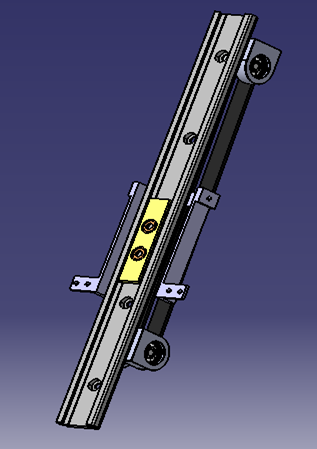
\includegraphics[scale=0.5]{chariot.png} 
	\caption{Mécanisme d'élévation}
\end{figure}
\end{frame}

\begin{frame}
\frametitle{Châssis et conceptions mécaniques}
\begin{figure}[!ht]
	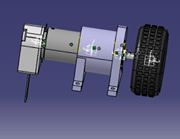
\includegraphics[scale=0.5]{support.jpg}
	\caption{Support moteur} 
\end{figure}
\end{frame}

\begin{frame}
\frametitle{Châssis et conceptions mécaniques}
\begin{figure}[!ht]
	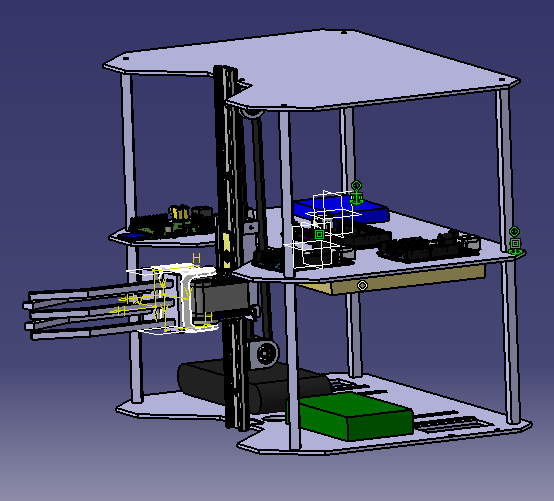
\includegraphics[scale=0.5]{assemblage.png}
	\caption{Assemblage des différents éléments} 
\end{figure}
\end{frame}

\begin{frame}
\frametitle{Châssis et conceptions mécaniques}
\framesubtitle{Inconvénients}
\begin{itemize}
	\item Une seule action à la fois;
	\item Le positionnement correct du robot face à l'objet;
	\item L'encombrement de la pince.
\end{itemize}
\end{frame}
